\documentclass[tikz,border=5pt]{standalone}
\usepackage[UTF8]{ctex}
\usepackage{amsmath,amssymb}
\usetikzlibrary{arrows.meta,calc}
\definecolor{ink}{HTML}{243447}\definecolor{blue}{HTML}{2765A2}
\definecolor{green}{HTML}{3F7D5B}\definecolor{red}{HTML}{B74739}
\tikzset{body/.style={draw=ink,thick},vec/.style={draw=blue,thick,-{Latex}},
guide/.style={gray!60,dashed},dim/.style={ink,{Latex}-{Latex}},
line cap=round,line join=round}
\newcommand{\starbody}[1]{
\shade[ball color=blue!9](0,0)circle(#1);
\draw[body](0,0)circle(#1);
\draw[blue,dashed](#1,0)arc(0:180:#1 and {#1*.28});
\draw[blue,line width=1.4pt](#1,0)arc(0:-180:#1 and {#1*.28});}
\begin{document}
\begin{tikzpicture}
\starbody{1.4}
\draw[guide](0,-1.4)--(0,1.4);
\draw[vec](0,1.65)--(0,2.25)node[above]{$z$};
\filldraw[fill=white,draw=red](0,1.4)circle(.065)node[left=5pt]{$-q$};
\filldraw[fill=white,draw=green](0,-1.4)circle(.065)node[left=5pt]{$+q$};
\fill[ink](0,0)circle(.03)node[below left]{$O$};
\draw[vec](1.4,0)--(1.4,1.0)node[right]{$B\boldsymbol e_z$};
\draw[dim](0,-1.9)--(1.4,-1.9)node[midway,below]{$r$};
\draw[blue](-1.12,-.24)--(-2,-.65)node[left]{赤道导电环};
\node at(0,-2.7){两极为等效源，环与恒星同缩};
\end{tikzpicture}
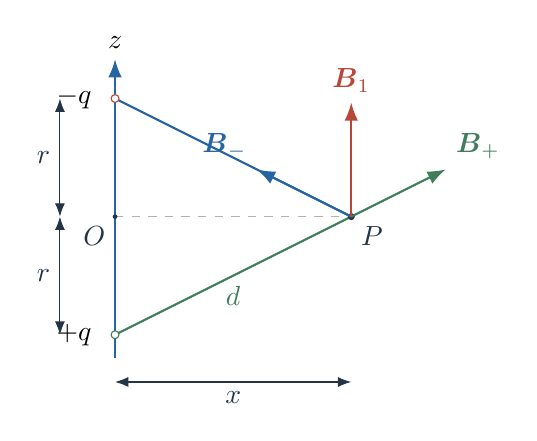
\begin{tikzpicture}
\coordinate(O)at(0,0);\coordinate(N)at(0,1.5);\coordinate(S)at(0,-1.5);\coordinate(P)at(3,0);
\draw[vec](0,-1.8)--(0,2.0)node[above]{$z$};
\draw[guide](O)--(P);
\draw[blue,thick](N)--(P);
\draw[green,thick](S)--(P)node[midway,below]{$d$};
\filldraw[fill=white,draw=red](N)circle(.05)node[left=5pt]{$-q$};
\filldraw[fill=white,draw=green](S)circle(.05)node[left=5pt]{$+q$};
\fill[ink](O)circle(.03)node[below left]{$O$};
\fill[ink](P)circle(.045)node[below right]{$P$};
\draw[green,thick,-{Latex}](P)--(4.2,.6)node[above right]{$\boldsymbol B_+$};
\draw[blue,thick,-{Latex}](P)--(1.8,.6)node[above left]{$\boldsymbol B_-$};
\draw[red,thick,-{Latex}](P)--(3,1.45)node[above]{$\boldsymbol B_1$};
\draw[dim](-.7,0)--(-.7,1.5)node[midway,left]{$r$};
\draw[dim](-.7,-1.5)--(-.7,0)node[midway,left]{$r$};
\draw[dim](0,-2.1)--(3,-2.1)node[midway,below]{$x$};
\end{tikzpicture}
\begin{tikzpicture}
\begin{scope}
\starbody{1.25}
\draw[vec](1.25,0)--(1.25,.6)node[right]{$B$};
\draw[dim](0,-1.65)--(1.25,-1.65)node[midway,below]{$r$};
\end{scope}
\begin{scope}[shift={(4.5,0)}]
\starbody{.75}
\draw[vec](.75,0)--(.75,1.6667)node[right]{$B_2=B/k^2$};
\draw[dim](0,-1.65)--(.75,-1.65)node[midway,below]{$R=kr$};
\end{scope}
\draw[vec](1.8,-.15)--(3.25,-.15)node[midway,above]{相似收缩};
\node[align=center]at(2.25,-2.65){面积尺度$\times k^2$\\$B_2R^2=Br^2$，随动磁通不变};
\end{tikzpicture}
\begin{tikzpicture}
\foreach\xx/\name in{0/感生项,4.8/运动项}{
\begin{scope}[shift={(\xx,0)}]
\draw[body](0,0)circle(1.25);
\draw[vec](1.25,0)--(.5,0)node[midway,below]{$\boldsymbol u$};
\node at(0,0){$\odot B_{\rm eq}$};
\node at(0,2.0){\name};
\end{scope}}
\draw[red,thick,-{Latex}](130:1.55)arc(130:20:1.55);
\begin{scope}[shift={(4.8,0)}]
\draw[green,thick,-{Latex}](20:1.55)arc(20:130:1.55);
\end{scope}
\node[align=center,text=red]at(0,-1.9){$\mathcal E_{\rm lab}=2\pi RaB_{\rm eq}<0$\\顺时针};
\node[align=center,text=green]at(4.8,-1.9){$\mathcal E_{\rm mot}=-2\pi RaB_{\rm eq}>0$\\逆时针};
\node at(2.4,-3.1){从$+z$方向看；$a<0$，总电动势为零};
\end{tikzpicture}
\end{document}
